\documentclass{beamer}
%
% Choose how your presentation looks.
%
% For more themes, color themes and font themes, see:
% http://deic.uab.es/~iblanes/beamer_gallery/index_by_theme.html
%
\mode<presentation>
{
  \usetheme{default}      % or try Darmstadt, Madrid, Warsaw, ...
  \usecolortheme{default} % or try albatross, beaver, crane, ...
  \usefonttheme{default}  % or try serif, structurebold, ...
  \setbeamertemplate{navigation symbols}{}
  \setbeamertemplate{caption}[numbered]
} 

\usepackage[english]{babel}
\usepackage[utf8x]{inputenc}
\usepackage{amssymb}

\DeclareMathOperator{\im}{im}
\DeclareMathOperator{\mat}{Mat}
\DeclareMathOperator{\rg}{rg}
\DeclareMathOperator{\id}{id}
\DeclareMathOperator{\gl}{Gl}
\DeclareMathOperator{\spl}{Sl}
\DeclareMathOperator{\cyl}{Cyl}
\DeclareMathOperator{\cone}{Cone}

% Macro definitions

\newcommand{\sphere}[1]{\mathbb{S}^{#1}}
\newcommand{\disk}[1]{\mathbb{D}^{#1}}
\newcommand{\interval}{\mathbb{I}}
\newcommand{\RP}[1]{\mathbb{RP}^{#1}}
\newcommand{\CP}[1]{\mathbb{CP}^{#1}}

% \H is already defined
\newcommand{\C}{\mathbb{C}}
\newcommand{\R}{\mathbb{R}}
\newcommand{\Z}{\mathbb{Z}}

\title{Motivation}
\author{Ben}
\institute{University of Bonn}
\date{\today}

%%%%%%%%%%%%%%%%%%%%%%%%%%%%%%%%%%%%%%%%%%%%%%%%%%%%%%%%%%%%%%%%%%%%%%%%%%%%%%
\begin{document}

%\begin{frame}
%  \titlepage
%\end{frame}

% Uncomment these lines for an automatically generated outline.
%\begin{frame}{Outline}
%  \tableofcontents
%\end{frame}

\section{Motivation}

\begin{frame}{$\CP{2}$ versus $\sphere{2} \vee \sphere{4}$}
	
	\begin{itemize}
	  \item $\CP{2} = $ ($0$-cell) $\cup$ ($2$-cell) $\cup_{\eta}$ ($4$-cell)
	  
	  \pause
	  
	  \item Question: What is the difference between $\sphere{2} \vee \sphere{4}$
	  and $\CP{2}$?
	  \item How can we prove that they are \textbf{not} homotopy equivalent?
	\end{itemize}
	
	\pause

	\renewcommand{\arraystretch}{1.3}
	\begin{table}
		\centering
		\begin{tabular}{c|c}
			$\CP{2}$ 			& $\sphere{2} \vee \sphere{4}$ \\\hline
			$\Z[x]/x^{3}$ 		& $\Z[\alpha, \beta]/(\alpha^2, \beta^2, \alpha \beta)$ \\
			$|x| = 2$ 			& $|\alpha| = 2, |\beta| = 4$
		\end{tabular}
		\caption{\label{tab:cup_producs} Cup product structures on $H^{*}(\underline{\quad}; \Z)$.}
	\end{table}

\end{frame}


\begin{frame}{The Hopf map}

	\begin{itemize}
		\item The attaching map of the $4$-cell,
		\[
			\eta \colon \partial \disk{4} = \sphere{3} \rightarrow \sphere{2} = \textrm{2-skeleton of } \CP{2}
		\]
		is called the \textit{Hopf map}.
		
		\pause
		
		\item In other words, $\CP{2} = \operatorname{Cone}(\eta)$ is
		the mapping cone of the Hopf map.
		\item The argument on the last slide shows that $\eta$ is not nullhomotopic,
		$0 \ne [\eta] \in \pi_3(\sphere{2})$, because if it were zero its mapping cone would
		be homotopy equivalent to $\sphere{2} \vee \sphere{4}$.
		
		\pause
		
		\item One explicit way to think of this map is by writing it as
		\begin{align*}
			\C^{2} \supset \sphere{3} & \rightarrow \C \cup \{ \infty \} = \CP{1} \\
						   (z_0, z_1) & \mapsto \frac{z_0}{z_1}
		\end{align*}
	\end{itemize}

\end{frame}


\begin{frame}{Hopf fibration}
	\begin{figure}
		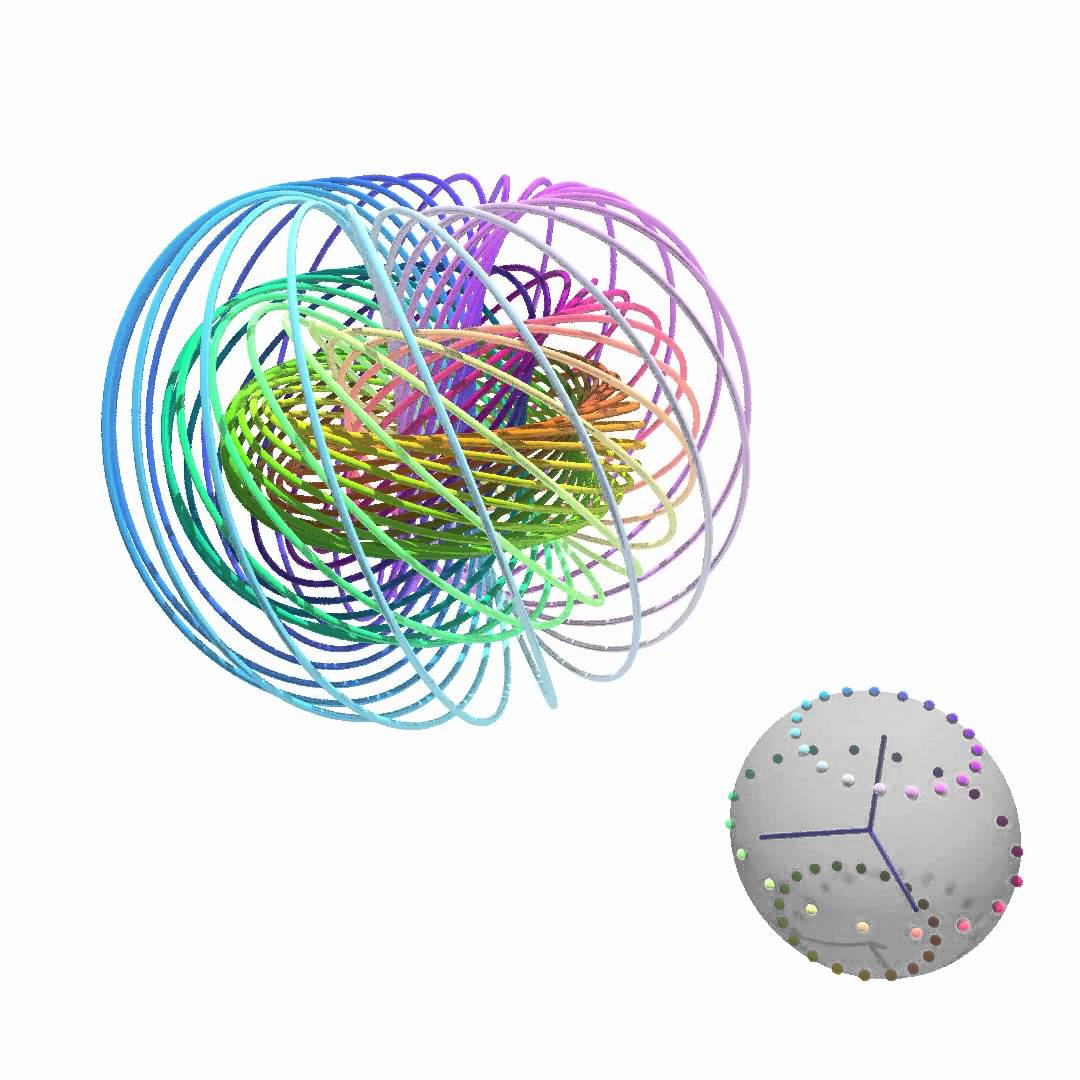
\includegraphics[width=0.6\textwidth]{pictures/hopf_fibration.jpg}
		\caption{
			\label{fig:hopf_fibration}
			Some fibres of $\eta \colon \sphere{3} \rightarrow \sphere{2}$
			drawn in $\sphere{3} = \R^{3} \cup \{ \infty \}$ \newline
			Source: \url{https://nilesjohnson.net/hopf-production.html}}
	\end{figure}
\end{frame}


\section{Stable setting}

\begin{frame}{Outlook on the next semester: Stable phenomena}

	\begin{itemize}
		\item What about $\Sigma \CP{2} = $ ($0$-cell) $\cup$ ($3$-cell) $\cup_{\Sigma \eta}$ ($5$-cell)?
		\pause
		\item Is $\Sigma \CP{2}$ homotopy equivalent to $\sphere{3} \vee \sphere{5}$?
		\pause
		\item Cup products are of no help here since they are trivial
		on a suspension! (Why?)
	\end{itemize}
	
	\pause
	\vfill
	
	\begin{block}{We will also look at the (iterated) suspensions:}
		\begin{align*}
			\eta \colon \sphere{3} & \rightarrow \sphere{2} \in \pi_3(\sphere{2}) \\
			\leadsto \Sigma \eta \colon \sphere{4} & \rightarrow \sphere{3} \in \pi_4(\sphere{3}) \\
			\leadsto \Sigma^{2} \eta \colon \sphere{5} & \rightarrow \sphere{4} \in \pi_5(\sphere{4}) \\
			\leadsto \ldots
		\end{align*}
	\end{block}

\end{frame}

\section{Homotopy groups of spheres}

\begin{frame}{Homotopy groups of spheres}

	\begin{figure}
		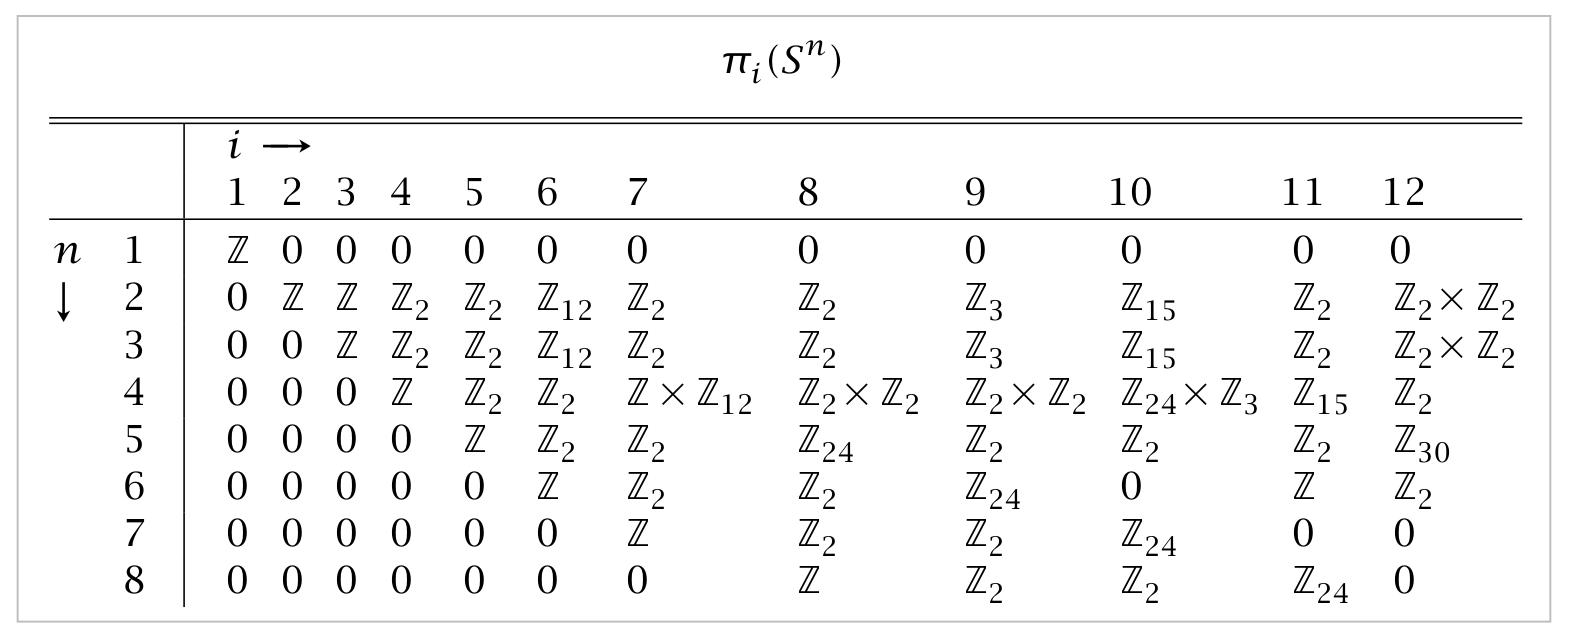
\includegraphics[width=\textwidth]{pictures/spheres_homotopy_groups.png}
		\caption{
			\label{fig:spheres_homotopy_groups}
			Some homotopy groups of spheres. \newline
			Source: Hatcher, Algebraic Topology, Section 4.1, p.339}
	\end{figure}

\end{frame}

\end{document}
